\documentclass{article}

% Default packages
\usepackage[utf8]{inputenc}
\usepackage[spanish]{babel}
\usepackage{fancyhdr}
\usepackage{tikz}
\usepackage{amssymb}
\usepackage{float}

\usepackage{listings}
\usepackage{xcolor}

\lstset{
    showstringspaces=false, % don't mark spaces in strings
    numbers=left, % display line numbers on the left
    commentstyle=\color{blue}, % comment color
    keywordstyle=\color{magenta}, % keyword color
    stringstyle=\color{red} % string color
}

\usepackage{color}
\definecolor{lightgray}{rgb}{0.95, 0.95, 0.95}
\definecolor{darkgray}{rgb}{0.4, 0.4, 0.4}
%\definecolor{purple}{rgb}{0.65, 0.12, 0.82}
\definecolor{editorGray}{rgb}{0.95, 0.95, 0.95}
\definecolor{editorOcher}{rgb}{1, 0.5, 0} % #FF7F00 -> rgb(239, 169, 0)
\definecolor{editorGreen}{rgb}{0, 0.5, 0} % #007C00 -> rgb(0, 124, 0)
\definecolor{orange}{rgb}{1,0.45,0.13}		
\definecolor{olive}{rgb}{0.17,0.59,0.20}
\definecolor{brown}{rgb}{0.69,0.31,0.31}
\definecolor{purple}{rgb}{0.38,0.18,0.81}
\definecolor{lightblue}{rgb}{0.1,0.57,0.7}
\definecolor{lightred}{rgb}{1,0.4,0.5}
\usepackage{upquote}
\usepackage{listings}
% JavaScript
\lstdefinelanguage{JavaScript}{
  morekeywords={typeof, new, true, false, catch, function, return, null, catch, switch, var, if, in, while, do, else, case, break},
  morecomment=[s]{/*}{*/},
  morecomment=[l]//,
  morestring=[b]",
  morestring=[b]'
}

\usepackage{graphicx}
\graphicspath{ {./imagenes/} }

\usepackage{geometry}
\geometry{margin=2cm}

\title{Autómata}
\author{Axel Treviño Palacios} 
\date{22 de noviembre de 2020}
\def\thenumber{4}

\makeatletter
\let\thetitle\@title
\let\theauthor\@author
\let\thedate\@date
\makeatother

\pagestyle{fancy}
\fancyhead{}
\fancyfoot{}
\fancyfoot[R]{\thepage}
\fancyfoot[L]{\thetitle}
\renewcommand{\headrulewidth}{0pt}
\renewcommand{\footrulewidth}{0.5pt}

\begin{document}
	\begin{titlepage}
		\centering	 
	 	
	 	\begin{tikzpicture}[remember picture, overlay]
			\node[anchor=north east,inner sep=1cm] at (current page.north east)
				{
\includegraphics[height=3.5cm]{logoEscom}};
			\node[anchor=north west,inner sep=1cm] at (current page.north west)
				{
\includegraphics[height=3.5cm]{logoPoli}};
		\end{tikzpicture}

		\vspace{4cm}
		{\Large \scshape Instituto Politécnico Nacional \par}
		\vspace{1cm}

		{\rmfamily \bfseries \Large Escuela Superior de Cómputo \par}
		\vspace{4cm}

		{\itshape\Large Práctica \#\thenumber \par}
		\vspace{0.5cm}
		
		{\scshape\Huge \thetitle \par}
		\vspace{5cm}
			
		{\itshape\Large \theauthor \par}
		2CM5
		
		\thedate				
		
		\vfill
	\end{titlepage}

	\section{Objetivo}
	Hacer la transformación del NFA al DFA que busca las palabras ``web'' y ``ebay''. Realizar el proceso utilizando los subconjuntos y sus relaciones.
	
	\section{Proceso de conversión}
	\begin{itemize}
	\item Primero la tabla de conversión de no determinístico a determinístico:

		\begin{itemize}
  	  	\item Inicié el proceso ignorando todas las islas del grafo completo y solamente anotando los nodos que se presentaran dentro del siguiente paso.
	
		\item Continué procesando los nodos iniciales y los nodos que siguieran hasta que no se generara ningún otro nodo.

		\item Después señalé cada condición que no se conectara a 1, y con esa información detecté el conjunto de excepciones $\{x\}$ en la fórmula $\Sigma-\{x\}$ de la conexión al primer nodo.
		
		\item Finalizando marqué con \textbf{negritas} todos los nodos finales.
		\end{itemize}
		
	\item Segundo la creación del grafo:

		\begin{itemize}
  	  	\item Para empezar creé todos los nodos y los puse desordenados en el canvas.
  	  	
  	  	\item Posterior a eso puse en su lugar todas las conexiones dictadas por la tabla, sin aún poner los elementos dentro de las flechas.
  	  	
  	  	\item Proseguí estableciendo el contenido a cada una de las flechas siguiendo las instrucciones del catálogo de conversión.
		
  	  	\item Concluí acomodando todos los nodos y flechas para aminorar el bullicio de lineas y letras.  	  	
  	  	\end{itemize}
	
	\end{itemize}
	
	\begin{figure}[h]
    \centering
    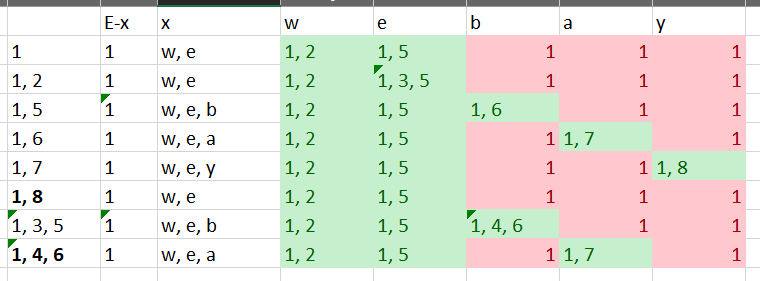
\includegraphics[width=0.75\textwidth]{Proceso}
    \caption{Tabla de Conversión}
    \label{fig:proceso}
	\end{figure}
	
	\newpage
	\section{Resultado}
	Y aquí se ve el resultado de la tabla de conversión \textit{(Figura \ref{fig:proceso})}.\par
	
\begin{figure} [H]
\begin{center}

\begin{tikzpicture}[scale=0.2]
\tikzstyle{every node}+=[inner sep=0pt]
\draw [black] (14.6,-28.5) circle (3);
\draw (14.6,-28.5) node {$1$};
\draw [black] (31.3,-19.9) circle (3);
\draw (31.3,-19.9) node {$1,\mbox{ }2$};
\draw [black] (31.3,-37.4) circle (3);
\draw (31.3,-37.4) node {$1,\mbox{ }5$};
\draw [black] (45.6,-37.4) circle (3);
\draw (45.6,-37.4) node {$1,\mbox{ }6$};
\draw [black] (59.9,-37.4) circle (3);
\draw (59.9,-37.4) node {$1,\mbox{ }7$};
\draw [black] (72.6,-37.4) circle (3);
\draw (72.6,-37.4) node {$1,\mbox{ }8$};
\draw [black] (72.6,-37.4) circle (2.4);
\draw [black] (45.6,-19.9) circle (3);
\draw (45.6,-19.9) node {$1,\mbox{ }3,\mbox{ }5$};
\draw [black] (59.9,-19.9) circle (3);
\draw (59.9,-19.9) node {$1,\mbox{ }4,\mbox{ }6$};
\draw [black] (59.9,-19.9) circle (2.4);
\draw [black] (17.27,-27.13) -- (28.63,-21.27);
\fill [black] (28.63,-21.27) -- (27.69,-21.2) -- (28.15,-22.08);
\draw (24.16,-24.7) node [below] {$w$};
\draw [black] (17.25,-29.91) -- (28.65,-35.99);
\fill [black] (28.65,-35.99) -- (28.18,-35.17) -- (27.71,-36.05);
\draw (23.89,-32.45) node [above] {$e$};
\draw [black] (31.681,-22.864) arc (35.0669:-252.9331:2.25);
\draw (28.01,-26.83) node [below] {$w$};
\fill [black] (29.18,-22.01) -- (28.24,-22.06) -- (28.81,-22.87);
\draw [black] (34.3,-19.9) -- (42.6,-19.9);
\fill [black] (42.6,-19.9) -- (41.8,-19.4) -- (41.8,-20.4);
\draw (38.45,-20.4) node [below] {$e$};
\draw [black] (33.011,-22.357) arc (28.36219:-28.36219:13.248);
\fill [black] (33.01,-22.36) -- (32.95,-23.3) -- (33.83,-22.82);
\draw (35.1,-28.65) node [right] {$w$};
\draw [black] (34.3,-37.4) -- (42.6,-37.4);
\fill [black] (42.6,-37.4) -- (41.8,-36.9) -- (41.8,-37.9);
\draw (38.45,-36.9) node [above] {$b$};
\draw [black] (33.472,-17.851) arc (123.73447:56.26553:8.963);
\fill [black] (33.47,-17.85) -- (34.42,-17.82) -- (33.86,-16.99);
\draw (38.45,-15.84) node [above] {$w$};
\draw [black] (34.064,-18.737) arc (110.23657:69.76343:33.35);
\fill [black] (34.06,-18.74) -- (34.99,-18.93) -- (34.64,-17.99);
\draw (45.6,-16.18) node [above] {$w$};
\draw [black] (43.102,-39.044) arc (-64.58398:-115.41602:10.839);
\fill [black] (33.8,-39.04) -- (34.31,-39.84) -- (34.74,-38.94);
\draw (38.45,-40.59) node [below] {$e$};
\draw [black] (57.187,-38.677) arc (-67.61111:-112.38889:30.421);
\fill [black] (34.01,-38.68) -- (34.56,-39.44) -- (34.94,-38.52);
\draw (45.6,-41.47) node [below] {$e$};
\draw [black] (69.761,-38.37) arc (-72.58253:-107.41747:59.504);
\fill [black] (34.14,-38.37) -- (34.75,-39.09) -- (35.05,-38.13);
\draw (51.95,-41.6) node [below] {$e$};
\draw [black] (33.573,-21.858) arc (47.74088:30.76658:56.548);
\fill [black] (33.57,-21.86) -- (33.83,-22.77) -- (34.5,-22.03);
\draw (39.89,-26.5) node [right] {$w$};
\draw [black] (34.004,-21.199) arc (63.76303:53.31304:151.317);
\fill [black] (34,-21.2) -- (34.5,-22) -- (34.94,-21.1);
\draw (47.31,-27.36) node [above] {$w$};
\draw [black] (34.147,-20.846) arc (71.29314:62.77931:261.852);
\fill [black] (34.15,-20.85) -- (34.74,-21.58) -- (35.07,-20.63);
\draw (53.51,-27.25) node [above] {$w$};
\draw [black] (44.383,-22.641) arc (-26.24614:-52.26132:37.351);
\fill [black] (33.74,-35.66) -- (34.68,-35.57) -- (34.07,-34.78);
\draw (40.36,-31.19) node [right] {$e$};
\draw [black] (57.561,-21.779) arc (-51.94347:-65.1326:120.069);
\fill [black] (34.04,-36.17) -- (34.97,-36.29) -- (34.55,-35.38);
\draw (47.16,-30.15) node [below] {$e$};
\draw [black] (48.6,-37.4) -- (56.9,-37.4);
\fill [black] (56.9,-37.4) -- (56.1,-36.9) -- (56.1,-37.9);
\draw (52.75,-36.9) node [above] {$a$};
\draw [black] (62.9,-37.4) -- (69.6,-37.4);
\fill [black] (69.6,-37.4) -- (68.8,-36.9) -- (68.8,-37.9);
\draw (66.25,-36.9) node [above] {$y$};
\draw [black] (48.6,-19.9) -- (56.9,-19.9);
\fill [black] (56.9,-19.9) -- (56.1,-19.4) -- (56.1,-20.4);
\draw (52.75,-20.4) node [below] {$b$};
\draw [black] (59.9,-22.9) -- (59.9,-34.4);
\fill [black] (59.9,-34.4) -- (60.4,-33.6) -- (59.4,-33.6);
\draw (59.4,-28.65) node [left] {$a$};
\draw [black] (29.125,-35.351) arc (254.44979:-33.55021:2.25);
\draw (28.06,-30.55) node [above] {$e$};
\fill [black] (31.6,-34.43) -- (32.3,-33.79) -- (31.34,-33.52);
\draw [black] (12.888,-26.05) arc (-153.83201:-331.67377:9.794);
\fill [black] (12.89,-26.05) -- (12.98,-25.11) -- (12.09,-25.55);
\draw (14.27,-12.51) node [above] {$\Sigma-w-e$};
\draw [black] (29.918,-40.049) arc (-36.51264:-199.59671:9.592);
\fill [black] (13.17,-31.12) -- (12.43,-31.71) -- (13.37,-32.05);
\draw (13.94,-43.32) node [below] {$\Sigma-w-e-b$};
\draw [black] (43.953,-39.903) arc (-38.55523:-173.48197:16.493);
\fill [black] (14.67,-31.5) -- (14.26,-32.35) -- (15.26,-32.23);
\draw (23.49,-46.18) node [below] {$\Sigma-w-e-a$};
\draw [black] (58.354,-39.968) arc (-34.62541:-167.60502:24.058);
\fill [black] (15.06,-31.46) -- (14.74,-32.35) -- (15.72,-32.14);
\draw (31.85,-50.74) node [below] {$\Sigma-w-e-y$};
\draw [black] (70.168,-39.155) arc (-56.31451:-141.13327:40.333);
\fill [black] (16.39,-30.9) -- (16.51,-31.84) -- (17.29,-31.21);
\draw (40.54,-46.24) node [below] {$\Sigma-w-e$};
\draw [black] (14.203,-25.531) arc (-177.72442:-331.26549:16.101);
\fill [black] (14.2,-25.53) -- (14.67,-24.71) -- (13.67,-24.75);
\draw (23.01,-8.66) node [above] {$\Sigma-w-e-b$};
\draw [black] (16.143,-25.929) arc (146.12283:55.37602:29.59);
\fill [black] (16.14,-25.93) -- (17,-25.54) -- (16.17,-24.99);
\draw (33.24,-12.52) node [above] {$\Sigma-w-e-a$};
\draw [black] (11.92,-29.823) arc (324:36:2.25);
\draw (7.35,-28.5) node [left] {$\Sigma-w-e$};
\fill [black] (11.92,-27.18) -- (11.57,-26.3) -- (10.98,-27.11);
\end{tikzpicture}

\end{center}
\caption{Grafo del Autómata Finito Determinístico}
\end{figure}


\end{document}